\chapter*{2018年\textsf{HDU}「大学物理1」期中试题解答}

\begin{minipage}{0.32\textwidth}
    \textbf{开课学院}：理学院
      
    \textbf{课程编码}：A0715011
\end{minipage}
\hfill
\begin{minipage}{0.32\textwidth}
    \textbf{解析制作}：\textsf{M.Xia@WeYoung}

    \textbf{\,\hologo{TeX}~排版}：\textsf{M.Xia}
\end{minipage}
\hfill
\begin{minipage}{0.15\textwidth}
    \centering
    \begin{tikzpicture}
        \node [inner sep=0] at (0,0) {
            \qrcode[height=3em,version=4]{https://qm.qq.com/q/mgD30uPiSs}};
        \fill [color=white,rounded corners=(sqrt(2)+2)/11*1em] (-.5em,-.5em) rectangle (.5em,.5em);
        \node [inner sep=0] at (0,0) {\color{MidnightBlue}\scriptsize\faIcon{qq}};
    \end{tikzpicture}

    \scriptsize\href{https://qm.qq.com/q/mgD30uPiSs}{\itshape 未央物理营}
\end{minipage}
\hfill
\begin{minipage}{0.15\textwidth}
    \centering
    \begin{tikzpicture}
        \node [inner sep=0] at (0,0) {
            \qrcode[height=3em,version=4]{http://weixin.qq.com/r/DBIABcHEqgnWKIVmb0eI}};
            \fill [color=white,rounded corners=(sqrt(2)+2)/11*1em] (-.5em,-.5em) rectangle (.5em,.5em);
        \node [inner sep=0] at (0,0) {\color{DarkGreen}\scriptsize\faIcon{weixin}};
    \end{tikzpicture}

    \scriptsize\href{http://weixin.qq.com/r/DBIABcHEqgnWKIVmb0eI}{\itshape 未央学社}
\end{minipage}

\section{选择题（每题3分，共30分）}

\begin{problem}
    某质点作直线运动的运动学方程为$x=2t-6t^2+7$ (SI)，则该质点作
    \begin{tasks}(2)
        \task 匀加速直线运动，加速度沿$x$轴正方向
        \task[\true] 匀加速直线运动，加速度沿$x$轴负方向
        \task 变加速直线运动，加速度沿$x$轴正方向
        \task 变加速直线运动，加速度沿$x$轴负方向
    \end{tasks}
\end{problem}
\solute2
\begin{solution}
    质点的加速度$a=\d^2x/\d t^2=12$ (SI)为一大于零常数.
\end{solution}

\begin{problem} % {牛顿运动定律}
\begin{paracol}{2}
    质量分别为$m_1$和$m_2$的两滑块$A$和$B$通过一轻弹簧水平连结后置于水平桌面上，滑块与桌面间的摩擦系数为$\mu$，系统在水平拉力$F$作用下匀速运动，如图所示. 如突然撤销拉力，则刚撤销后瞬间，二者的加速度$a_A$和$a_B$分别为
    \switchcolumn\vspace*{\fill}\centering
    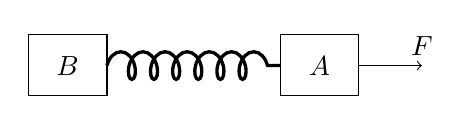
\begin{tikzpicture}
        \wall{(-2.5,0)}{(2.5,-.2)};
        \draw (-2.2,.02) rectangle (-1.2,.8);
        \draw [very thick,decoration={aspect=.6, segment length=8, amplitude=5,coil},decorate] (-1.2,.4) -- (1,.4); %amplitude调整螺线管的直径，segment length调整间距
        \draw (1,.02) rectangle (2,.8);
        \draw [->] (2,.4) -- (2.8,.4) node [anchor=south] {$F$};
        \node at (-1.7,.4) {$B$};
        \node at (1.5,.4) {$A$};
    \end{tikzpicture}\vspace*{\fill}
\end{paracol}
\begin{tasks}(4)
    \task $a_A=0$，$a_B=0$
    \task $a_A>0$，$a_B<0$
    \task $a_A<0$，$a_B>0$
    \task[\true] $a_A<0$，$a_B=0$
\end{tasks}
\end{problem}
\solute3
\begin{solution}
    撤掉$F$后弹簧弹力不会立刻消失，故$B$仍然保持着匀速运动的状态，$a_B=0$；$A$只受到向左的弹簧弹力和摩擦力，故其做减速运动，$a_A<0$.
\end{solution}

\begin{paracol}{2}
\begin{problem} % 功
    如图所示，木块$m$沿固定的光滑斜面下滑，当下降$h$高度时，重力做功的瞬时功率是
    \begin{tasks}(2)
        \task[\true] $mg\sin\theta\sqrt{2gh}$
        \task $mg\cos\theta\sqrt{2gh}$
        \task $mg\sin\sqrt{gh/2}$
        \task $mg\sqrt{gh/2}$
    \end{tasks}
\switchcolumn\vspace*{\fill}\centering
\begin{tikzpicture}
    \draw (4,0) coordinate (a) -- (0,0) coordinate (o) -- (3.2,2.4) coordinate (b);
    \draw [rotate=36.8,densely dashed] (.5,0) -- (1.3,0) -- (1.3,.5) -- (.5,.5)--cycle;
    \draw [rotate=36.8] (2.3,0) -- (3.1,0) -- (3.1,.5) -- (2.3,.5)--cycle;
    \pic["$\theta$", draw=DarkRed, very thick, angle eccentricity=1.35, angle radius=24]{angle=a--o--b};
\end{tikzpicture}\vspace*{\fill}
\end{problem}
\end{paracol}
\solute3
\begin{solution}
    下降高度$h$时速度大小$v=\sqrt{2gh}$. 重力做功的瞬时功率$P=\bm F\cdot\bm v=mg\sin\theta\sqrt{2gh}$.
\end{solution}

\begin{problem}
\begin{paracol}{2}
    如图所示，一个小物体，位于光滑的水平桌面上，与一绳的一端相连结，绳的另一端穿过桌面中心的小孔$O$. 该物体原以角速度$\omega$在半径为$R$的圆周上绕$O$旋转，今将绳从小孔缓慢往下拉. 则物体
    \switchcolumn\vspace*{\fill}\centering
    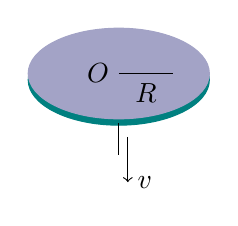
\begin{tikzpicture}[scale=1.15]
        \filldraw [yshift=-2,teal] (0,0) ellipse (1 and .5);
        \filldraw [MidnightBlue!40!] (0,0) ellipse (1 and .5);
        \draw (0,0) -- (.6,0);
        \draw (0,-.55) -- (0,-.9);
        \node [anchor=east] at (0,0) {$O$};
        \node [anchor=north] at (.3,0) {$R$};
        \draw [->] (.1,-.7) -- (.1,-1.2);
        \node [anchor=west] at (.1,-1.2) {$\bm v$};
    \end{tikzpicture}\vspace*{\fill}
\end{paracol}
\begin{tasks}(2)
    \task 动能不变，动量改变
    \task 动量不变，动能改变
    \task 角动量不变，动能不变
    \task[\true] 角动量不变，动能、动量都改变
\end{tasks}
\end{problem}
\solute2
\begin{solution}
    物体所受合力不等于零，动量改变. 受力始终指向$O$，其力矩为零，角动量不变. 下拉过程中物体运动半径减小，速度增大，动能变大.
\end{solution}

\begin{paracol}{2}
\begin{problem} % {动量定理}
    如图所示，质量为$m$的质点，沿正三角形$ABC$的水平光滑轨道匀速度$\bm v$运动，质点越过$A$点时，轨道作用于质点的冲量的大小
    \begin{tasks}(4)
        \task $mv$
        \task $\sqrt{2}mv$
        \task $\sqrt{3}mv$
        \task $2mv$
    \end{tasks}
\end{problem}
\switchcolumn\vspace*{\fill}\centering
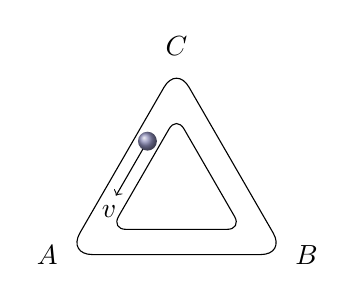
\begin{tikzpicture}[scale=.8]
    \draw [rounded corners=9] (0,2) node [above] {$C$} -- ({-sqrt(3)},-1) node [left] {$A$} -- ({sqrt(3)},-1) node [right] {$B$} -- cycle;
    \draw [scale=.6,rounded corners=5.4] (0,2) -- ({-sqrt(3)},-1) -- ({sqrt(3)},-1) -- cycle;
    \draw [->] ({-.8/sqrt(3)},.8) --++ (-.5,{-.5*sqrt(3)}) node [below,xshift=-sin(30)*.5em,] {$\bm v$};
    \shade [ball color=MidnightBlue!50] ({-.8/sqrt(3)},.8) circle (.15);
\end{tikzpicture}\vspace*{\fill}
\switchcolumn
\solute1
\begin{solution}
    $\abs{\Delta\bm p}=\abs{mv\bm i-\ab(-\frac12mv\bm i-\frac{\sqrt3}2mv\bm j)}=\sqrt3mv$.
\end{solution}
\end{paracol}

\begin{paracol}{2}
\begin{problem}
    竖直的圆筒形转筒，半径为$R$，绕中心轴$OO'$转动，物块$A$紧靠在圆筒的内壁上，物块与圆筒间的摩擦系数为$\mu$，要使物块$A$不下落，圆筒转动的角速度$\omega$至少应为
    \begin{tasks}(4)
        \task[\true] $\sqrt{g/\mu R}$
        \task $\sqrt{\mu gR}$
        \task $\sqrt{\mu/R}$
        \task $\sqrt{g/R}$
    \end{tasks}
\end{problem}
\switchcolumn\vspace*{\fill}\centering
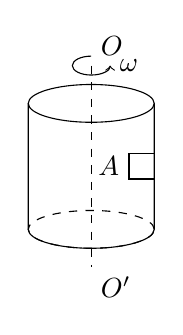
\begin{tikzpicture}[scale=.8]
    \draw (0,1) ellipse (1 and .3);
    \draw [dashed] (0,-1) ellipse (1 and .3);
    \draw (-1,1) -- (-1,-1) arc (-180:0:1 and .3) -- (1,1);
    \draw [dashed] (0,1.6) node [above right] {$O$} -- (0,-1.6) node [below right] {$O'$};
    \draw (1,.2) rectangle (.6,-.2) node [left] at (.6,0) {$A$};
    \draw [->] (0,1.75) arc (90:360:.3 and .15) node [right] {$\omega$};
\end{tikzpicture}\vspace*{\fill}
\switchcolumn
\solute1
\begin{solution}
    由$f=mg=\mu N$，$N=m\omega^2R$得$\omega=\sqrt{g/\mu R}$.
\end{solution}
\end{paracol}

\begin{problem}
    假设卫星环绕地球中心做圆周运动，则在运动过程中，卫星对地球中心的
    \begin{tasks}(3)
        \task[\true] 角动量守恒，动能也守恒
        \task 角动量守恒，动能不守恒
        \task 角动量不守恒，动能守恒
        \task 角动量不守恒，动量不守恒
        \task 角动量守恒，动量守恒
    \end{tasks}
\end{problem}
\begin{solution}
    卫星所受引力始终指向地球中心，所以引力力矩为零，角动量守恒；由于卫星做圆周运动，其与地球中心的距离保持不变，所以速度保持不变，所以动能守恒.
\end{solution}

\begin{problem}
    高斯定理$\oiint_S{\bm E\cdot\d\bm S}=\int_V{\frac{\rho}{\epsilon_0}\d V}$
    \begin{tasks}(2)
        \task[\true] 适用于任何静电场
        \task 只适用于真空中的静电场
        \task! 只适用于具有球对称性、周对称性和平面对称性的静电场
        \task! 只适用于虽然不具有C中所述的对称性、但可以找到合适的高斯面的静电场
    \end{tasks}
\end{problem}

\begin{problem}
    在边长为$a$的正方体中心处放置一电荷$Q$，则正方体顶角处的电场强度的大小为
    \begin{tasks}(4)
        \task $Q/12\pi\epsilon_0a^2$
        \task $Q/6\pi\epsilon_0a^2$
        \task[\true] $Q/3\pi\epsilon_0a^2$
        \task $Q/\pi\epsilon_0a^2$
    \end{tasks}
\end{problem}
\solute1
\begin{solution}
    $E=Q/4\pi\epsilon_0(\sqrt{3}a/2)^2=Q/3\pi\epsilon_0a^2$.
\end{solution}

\section{填空题（每题3分，共21分）}

\begin{problem}
    一物体在某瞬时，以初速度$\bm v_0$从某点开始运动，在$\Delta t$时间内，经一长度为$s$的曲线路径后，又回到出发点，此时速度为$-\bm v_0$，则在这段时间内，物体的平均速率是\ans{$s/\Delta t$}，物体的平均加速度是\ans{$-2\bm v_0/\Delta t$}.
\end{problem}

\begin{problem}
    一吊车底板上放一质量为$\qty{10}\kg$的物体，若吊车底板加速上升，加速度大小为$a=3+5t$ (SI)，则$\qty2\s$内吊车底板给物体的冲量大小$I=$\ans{$\qty{356}{\N\cdot\s}$}，$\qty2\s$内物体动量的增量大小$\Delta P=$\ans{$\qty{160}{\N\cdot\s}$}.
\end{problem}
\begin{solution}
    $v(2)=\int_0^2a\d t=\qty{16}{\m/\s}$，$I=m\Delta v+mgt=\qty{356}{\N\cdot\s}$，$\Delta P=m\Delta v=\qty{160}{\N\cdot\s}$.
\end{solution}

\begin{problem}
    哈雷慧星绕太阳的轨道是以太阳为一个焦点的椭圆. 它离太阳最近的距离是$r_1=\qty{8.75e10}\m$，此时它的速率是$v_1=\qty{5.46e4}{\m/\s}$. 它离太阳最远时的速率是$v_2=\qty{9.08e2}{\m/\s}$，这时它离太阳的距离是$r_2=$\ans{$\qty{5.26e12}\m$}.
\end{problem}
\solute0
\begin{solution}
    由彗星对太阳角动量守恒$mv_1r_1=mv_2r_2$得远日点距离$r_2=v_1r_1/v_2=\qty{5.26e12}\m$.
\end{solution}

\begin{paracol}{2}
\begin{problem}
    一半径为$R$的带有一缺口的细圆环，缺口长度为$d$（$d\ll R$）环上均匀带有正电，电荷为$q$，如图所示. 则圆心$O$处的场强大小为\ans{$qd/8\pi^2\epsilon_0R^3$}.
    \switchcolumn\vspace*{\fill}\centering
    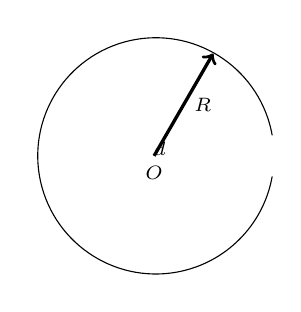
\begin{tikzpicture}[scale=1.5]
        \draw [yshift=sin(10)*1cm] (1,0) arc (10:350:1);
        \draw [very thick,->] (0,0) -- (.5,{sqrt(3)/2}) node [right,midway] {$\scriptstyle R$} node [at start,below] {$\scriptstyle O$};
        \length{(1.25,{sin(10)})}{(1.25,{-sin(10)})}{$\scriptstyle d$}{(0,-.75)};
    \end{tikzpicture}
    \vspace*{\fill}
\end{problem}
\switchcolumn
\solute2
\begin{solution}
    可等价用一带电量为$-q$的完整圆环叠加在此圆环上，此时只有缺口处存在电量$-qd/2\pi R$. 由于$d\ll R$，缺口处可看作点电荷. 圆心处的场强大小为$E=qd/8\pi^2\epsilon_0R^3$.
\end{solution}
\end{paracol}

\begin{problem}
    有一半径为$R$的匀质圆形水平转台，可绕通过盘心$o$且垂直于盘面的竖直固定轴$OO'$转动，转动惯量为$J$. 台上有一人，质量为$m$. 当他站在离转轴$r$处时（$r<R$），转台和人一起以$\omega_1$的角速度转动，如图. 若转轴处摩擦可以忽略，问当人走到转台边缘时，转台和人一起转动的角速度$\omega_2=$\ans{$(J+mr^2)\omega_1/(J+mR^2)$}.
\end{problem}
\solute0
\begin{solution}
    由角动量守恒$(mr^2+J)\omega_1=(mR^2+J)\omega_2$得$\omega_2=(J+mr^2)\omega_1/(J+mR^2)$.
\end{solution}

\section{计算题（共53分）}

\begin{paracol}{2}
\begin{problem} % {牛顿第二定律}
    如图左下所示，质量为$m$的摆球$A$悬挂在车架上. 求在下述各种情况下，摆球与竖直方向的夹角$\alpha$和线中的张力$T$.
    \begin{enumerate}
        \item 小车沿水平方向做匀速运动.
        \item 小车沿水平方向做加速度为$\bm a$的运动.
    \end{enumerate}
    \switchcolumn\vspace*{\fill}\centering
    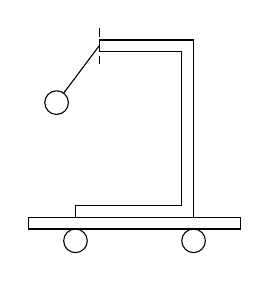
\begin{tikzpicture}[scale=.75]
        \wall{(-2,0)}{(2,-.3)};
        \draw (-1,.2) circle (.2);
        \draw (1,.2) circle (.2);
        \draw (-1.8,.4) rectangle (1.8,.6);
        \draw (-1,.6) -- (1,.6) -- (1,3.6) -- (-.6,3.6) -- (-.6,3.4) -- (.8,3.4) -- (.8,.8) -- (-1,.8) -- cycle;
        \draw [densely dashed] (-.6,3.8) -- (-.6,3.2);
        \draw (-.6,3.5) --++ (-.6,-.8) ++ (-.12,-.16) circle (.2);
    \end{tikzpicture}\vspace*{\fill}
\end{problem}
\end{paracol}
\solute1
\begin{solution}\leavevmode
    \begin{enumerate}
        \item 此时线处于竖直方向，此方向上摆球的受力平衡，即$\alpha=0$，$T=mg$.
        \item 引入惯性力$-m\bm a$,摆球分别在水平和竖直方向上受力平衡，即$T\sin\alpha=ma$，$T\cos\alpha=mg$，得$\alpha=\arctan{a/g}$，$T=m\sqrt{a^2+g^2}$.
    \end{enumerate}
\end{solution}

\begin{problem}
    有一质点沿$x$轴作直线运动，$t$时刻的坐标为$x=4.5t^2-2t^3$ (SI). 试求
    \begin{tasks}[label=\arabic*.](3)
        \task 第$2$秒内的平均速度.
        \task 第$2$秒末的瞬时速度.
        \task 第$2$秒内的路程.
    \end{tasks}
\end{problem}
\solute2
\begin{solution}\leavevmode
    \begin{tasks}[label=\arabic*.](2)
        \task $\bm{\overline v}=\Delta\bm x/\Delta t=-0.5\bm i\unit{\m/\s}$.
        \task $\bm v_2=\d\bm x/\d t\big|_{t=2}=9t\bm i-6t^2\bm i\big|_{t=2}=-6\bm i\unit{\m/\s}$.
        \task! $t=1.5$时，$x=0$. $s=\abs{x_{1.5}-x_1}+\abs{x_2-x_{1.5}}=\qty{2.25}\m$.
    \end{tasks}
\end{solution}

\begin{paracol}{2}
\begin{problem}
    如图所示，质量$m$为$\qty{0.1}\kg$的木块，在一个水平面上和一个劲度系数$k$为$\qty{20}{\N/\m}$的轻弹簧碰撞，木块将弹簧由原长压缩了$x=\qty{0.4}\m$. 假设木块与水平面间的滑动摩擦系数$\mu_k$为$0.25$，问在将要发生碰撞时木块的速率$v$为多少？
    \switchcolumn\vspace*{\fill}\centering
    \begin{tikzpicture}
        \draw [very thick,line cap=butt] (-2.5,0) -- (2.5,0) -- (2.5,1.5);
        \fill [pattern=north east lines] (-2.5,0) rectangle (2.5,-.2) rectangle (2.7,1.5);
        \draw (-2,0) rectangle (-1,.9) node [midway] {$m$};
        \draw [very thick,->] (-1.8,1.2) -- (-1.2,1.2);
        \draw [very thick] (0,0) -- (0,1.2);
        \draw [very thick,decoration={aspect=.6, segment length=6, amplitude=5,coil},decorate] (0,.5) -- (2.5,.5) node [midway,above,yshift=6pt] {$k$}; %amplitude调整螺线管的直径，segment length调整间距
    \end{tikzpicture}\vspace*{\fill}
\end{problem}
\end{paracol}
\solute0
\begin{solution}
    由动能定理$-\mu_kmgx-\int_0^xkx\d x=0-mv^2/2$得$v=\sqrt{2\mu_kgx+kx^2/m}=\qty{5.83}{\m/\s}$.
\end{solution}

\begin{problem} % {动量守恒}
    一电子和一个静止着的氢原子发生对心完全弹性碰撞. 已知氢原子质量为电子质量的$1840$倍，求碰撞过程中传给氢原子的能量与电子原来能量的比值.
\end{problem}
\solute2
\begin{solution}
    设电子质量为$m$，氢原子质量为$1840m$，电子速率为$v_0$. 碰撞过程中氢原子和电子组成的系统动量守恒
    \[mv_0=mv_1+1840mv_2\]
    由于碰撞为完全弹性碰撞，所以碰撞过程中能量守恒
    \[\frac12mv_0^2=\frac12mv_1^2+\frac12\cdot 1840 mv_2^2\]
    联立以上两式得$\Delta E_k/E_{k_0}=1840v_2^2/v_0^2=\num{2.17e-3}$.
\end{solution}

\begin{paracol}{2}
\begin{problem}
    一长为$\qty1\m$的均匀直棒可绕过其一端且与棒垂直的水平光滑固定轴转动. 抬起另一端使棒向上与水平面成$\qty{60}\degree$，然后无初转速地将棒释放. 已知棒对轴的转动惯量为$ml^2/3$，其中$m$和$l$分别为棒的质量和长度. 求
    \begin{enumerate}
        \item 放手时棒的角加速度.
        \item 棒转到水平位置时的角加速度.
    \end{enumerate}
    \switchcolumn\vspace*{\fill}\centering
    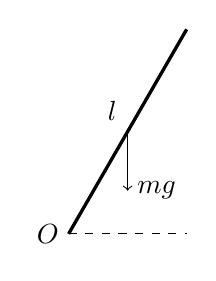
\begin{tikzpicture}[scale=1.5]
        \draw [dashed] (0,0) -- (1,0) node [at start,left] {$O$};
        \draw [very thick] (0,0) -- (1,{sqrt(3)}) node [midway,above left] {$l$};
        \draw [->] (.5,{sqrt(3)/2}) --++ (0,-.5) node [right] {$mg$};
    \end{tikzpicture}
    \vspace*{\fill}
\end{problem}
\end{paracol}
\solute1
\begin{solution}
    棒与水平面成任意角$\theta$时，其所受重力矩为$M=mgl\cos\theta/2$. 由转动定律$mgl\cos\theta/2=I\beta$得$\beta=3g\cos\theta/2l$. 其中$I=ml^2/3$为棒对轴的转动惯量.
    \begin{itemize}
        \item 放手时$\theta=\qty{60}\degree$，棒的角加速度$\beta=\qty{7.35}{\radian/\s^2}$.
        \item 棒转动到水平位置时$\theta=\qty{90}\degree$，棒的角加速度$\beta=\qty{14.7}{\radian/\s^2}$.
    \end{itemize}
\end{solution}

\begin{problem}
    两个无限长同轴柱圆柱面，半径分别为$R_1$，$R_2$（$R_2>R_1$）带有等值异号电荷，每单位长度的电量为$\lambda$，试求
    \begin{tasks}[label=\arabic*.](2)
        \task $r>R_2$时离轴线为$r$处的电场强度.
        \task $R_1<r<R_2$时离轴线为$r$处的电场强度.
    \end{tasks}
\end{problem}
\solute1
\begin{solution}\leavevmode
    \begin{enumerate}
        \item 取半径$r>R_2$，高度为$l$的圆柱高斯面，由高斯定理$E_1\cdot 2\pi rl=[+\lambda l+\ab(-\lambda)l]/\epsilon_0$得$E_1=0$.
        \item 取半径$R_1<r<R_2$，高度为$l$的圆柱高斯面，由高斯定理$E_2\cdot 2\pi rl=\lambda l/\epsilon_0$得$E_2=\lambda/2\pi r\epsilon_0$.
    \end{enumerate}
\end{solution}

\begin{paracol}{2}
\begin{problem}
    一轴承光滑的定滑轮，质量为$M=\qty{20.0}\kg$，半径为$R=\qty{0.10}\m$，一根不能伸长的轻绳，一端固定在定滑轮上，另一端系有一质量为$m=\qty{5.0}\kg$的物体，如左下图所示. 已知定滑轮的转动惯量为$J=MR^2/2$，其角速度$\omega_0=\qty{8.0}{\radian/\s}$，方向垂直纸面向里. 求
    \begin{enumerate}
        \item 定滑轮的角加速度.
        \item 定滑轮的角速度变化到$\omega=0$时，物体上升的高度.
        \item 当物体回到原来位置时，定滑轮的角速度.
    \end{enumerate}
    \switchcolumn\vspace*{\fill}\centering
    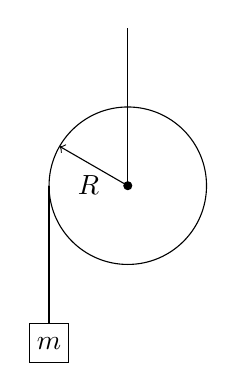
\begin{tikzpicture}
        \wall{(-1,0)}{(1,.2)};
        \draw (0,0) -- (0,-2);
        \draw (0,-2) circle (1);
        \draw (-1,-2) -- (-1,-3.75); 
        \draw (-1.25,-4.25) rectangle + (.5,.5) node [midway] {$m$};
        \filldraw (0,-2) circle (.05);
        \draw [->] (0,-2) -- ({-sqrt(3)/2},-1.5);
        \node [anchor=north] at (-.5,-1.75) {$R$};
    \end{tikzpicture}
    \vspace*{\fill}
\end{problem}
\end{paracol}
\solute2
\begin{solution}\leavevmode
    \begin{enumerate}
        \item 设绳子拉力为$T$. 对物块列牛顿运动定律、对滑轮列转动定律
        \[\begin{cases}
            mg-T=ma\\
            TR=MR^2\beta/2
        \end{cases}\]
        利用关系$a=R\beta$解得$\beta=-2mg/R(M+2m)=\qty{-32.7}{\radian/\s^2}$.
        \item 由$\omega^2-\omega_0^2=2\beta\theta$得$\theta=-\omega_0^2/2\beta=\qty{0.98}\radian$，$h=R\theta=\qty{0.098}\m$.
        \item 全过程无摩擦，保守力做功为零，所以定滑轮的角速度大小仍为$\omega_0=\qty8{\radian/\s}$，方向反向.
    \end{enumerate}
\end{solution}

\begin{paracol}{2}
\begin{problem}
    一段半径为$a$的细圆弧，对圆心的张角为$\theta$，其上均匀分布有正电荷$q$，如右上图所示. 试以$a$，$q$，$\theta$表示出圆心$O$处的电场强度.
    \switchcolumn\vspace*{\fill}\centering
    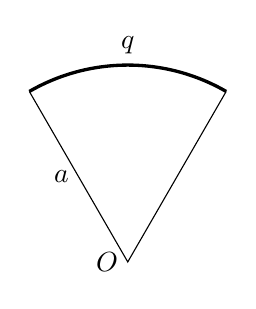
\begin{tikzpicture}[scale=2.5]
        \draw [very thick] (-.5,{.5*sqrt(3)}) arc (120:60:1) node [midway,above] {$q$};
        \draw (-.5,{.5*sqrt(3)}) -- (0,0) node [midway,left] {$a$} node [left] {$O$} -- (.5,{.5*sqrt(3)});
    \end{tikzpicture}\vspace*{\fill}
\end{problem}\switchcolumn
\solute2
\begin{solution}
    由对称性可得$O$处的电场强度沿$y$轴负方向. 取$\alpha\sim\alpha+\d\alpha$张角对应的线元，对其在$O$处产生的场强积分得$E=\int_{-\theta/2}^{\theta/2}-q\cos\alpha\d\alpha/4\pi\epsilon_0a^2\theta=-q\sin(\theta/2)/2\pi\epsilon_a^2\theta$.
\end{solution}
\end{paracol}